\section{Planetary Radar Sounders}
\label{sec:planetary_radar_sounders}
Planetary Radar Sounders (RS) are nadir-looking, low-frequency radar instruments specifically designed to probe the shallow subsurface of planetary bodies from orbit.
By transmitting short radio pulses in the HF–VHF bands (typically in the range 1–30~MHz) and recording the time-delayed echoes, RS instruments acquire  radargrams that represent the dielectric structure along the spacecraft ground track.
In contrast to Synthetic Aperture Radar (SAR) systems, which operate at higher frequencies and synthesize an along-track aperture to image surface backscatter, Radar Sounders trade azimuth resolution for increased penetration depth .

Representative examples of orbital Radar Sounders include MARSIS\cite{Jordan_2009} (Mars Advanced Radar for Subsurface and Ionosphere Sounding) on board \emph{Mars Express}\cite{ESA_MarsExpress} and SHARAD (SHAllow RADar)\cite{Seu_2007} on board \emph{Mars Reconnaissance Orbiter}\cite{Zurek_2007}.
Both instruments have demonstrated the capability to detect subsurface layering, buried basins, and potential volatile reservoirs on Mars, and similar sounders have been proposed or deployed for other planetary bodies.
In this work, we specifically focus on SHARAD, whose data are described in detail in Section~\ref{sec:dataset}, but the physical principles outlined below apply more generally to planetary RS systems.

\subsection{Electromagnetic Wave Propagation}
\label{subsec:em_propagation}
Radar Sounders operate by exploiting the interaction between electromagnetic waves and dielectric materials, which governs both wave propagation and echo formation.
The propagation of a radar signal through a medium is governed by its complex dielectric permittivity $\epsilon^*$, defined as:
\begin{equation}
\epsilon^* = \epsilon' - j\epsilon''
\end{equation}
where $\epsilon'$ is the real part (dielectric constant), which controls the phase velocity of the wave and thus the apparent depth of reflectors, and $\epsilon''$ is the imaginary part (dielectric loss factor), which controls the attenuation of the signal amplitude, and therefore the reflected power that can be measured at a given depth.

The velocity $v$ of the electromagnetic wave in a medium is given by:
\begin{equation}
v = \frac{c}{\sqrt{\epsilon'}}
\end{equation}
where $c \approx 3 \times 10^8$~m/s is the speed of light in vacuum.
This relationship is crucial for converting the temporal delay of radar echoes into geometric depth: a given sampling interval in time $\Delta t$ corresponds to a range sampling interval
\begin{equation}
\Delta r = \frac{v}{2}\,\Delta t = \frac{c}{2\sqrt{\epsilon'}}\,\Delta t,
\end{equation}
where the factor $1/2$ accounts for the two-way travel path (down and up).

Typical values of $\epsilon'$ and the corresponding phase velocities are reported below:
\begin{itemize}
    \item \textbf{Air / Vacuum:} $\epsilon' \approx 1$, $v \approx c \approx 3.0 \times 10^8$~m/s.
    \item \textbf{Liquid water:} $\epsilon' \approx 80$ at radio frequencies, $v \approx 3.3 \times 10^7$~m/s.
    \item \textbf{Pure water ice:} $\epsilon' \approx 3.1$–$3.2$, $v \approx 1.7 \times 10^8$~m/s.
    \item \textbf{Basaltic rock / dry regolith:} $\epsilon' \approx 4$–$8$ (depending on porosity and composition), $v \approx (1.1$–$1.5) \times 10^8$~m/s.
\end{itemize}

\begin{table}[t]
    \centering
    \caption{Typical values of relative dielectric permittivity $\epsilon'$ and corresponding phase velocity $v$ for materials relevant to planetary Radar Sounder applications.}
    \label{tab:dielectric_constants}
    \begin{tabular}{lcc}
        \hline
        Material                & $\epsilon'$ (–) & $v$ [m/s] \\
        \hline
        Vacuum / Air            & $\approx 1.0$   & $\approx 3.0 \times 10^8$ \\
        Liquid water            & $\approx 80$    & $\approx 3.3 \times 10^7$ \\
        Pure water ice          & $\approx 3.1$–$3.2$ & $\approx 1.7 \times 10^8$ \\
        Dry basaltic rock       & $\approx 6$–$8$ & $\approx (1.1$–$1.2) \times 10^8$ \\
        Porous dry regolith     & $\approx 3$–$5$ & $\approx (1.3$–$1.7) \times 10^8$ \\
        Ice–dust mixtures (Mars)& $\approx 3$–$6$ & $\approx (1.2$–$1.7) \times 10^8$ \\
        \hline
    \end{tabular}
\end{table}

On Mars, the shallow subsurface is expected to consist of mixtures of basaltic material, dust, and water ice, leading to effective dielectric constants in the range $\epsilon' \approx 3$–$6$ for many geologic units.
As a consequence, the apparent depth corresponding to a given time delay can vary significantly between terrains dominated by ice (higher velocity, larger depth per sample) and those dominated by rock or dust (lower velocity, smaller depth per sample).

\subsection{Reflection and Transmission}
When the propagating wave encounters an interface between two layers with different dielectric constants ($\epsilon'_1$ and $\epsilon'_2$), a portion of the electromagnetic energy is reflected back towards the Radar Sounder and a portion is transmitted into the second medium.
The first interface encountered is invariably between vacuum/air ($\epsilon'_1 \approx 1$) and the planetary surface material ($\epsilon'_2 \gg 1$), producing a strong reflection due to the large dielectric contrast.
Subsequent subsurface interfaces typically exhibit weaker contrasts.
For normal incidence, the amplitude of the reflected field is determined by the Fresnel reflection coefficient $R$:
\begin{equation}
R = \frac{\sqrt{\epsilon'_1} - \sqrt{\epsilon'_2}}{\sqrt{\epsilon'_1} + \sqrt{\epsilon'_2}}.
\end{equation}
A strong reflection (large $|R|$) implies a significant contrast in dielectric properties (e.g., ice/basalt interface), while weak reflections suggest gradual transitions or similar materials.

The fraction of power that is not reflected at the interface is transmitted into the second medium.
However, during propagation in this medium, the transmitted energy can be progressively reduced by several mechanisms, including material absorption (related to $\epsilon''$), volume scattering from inhomogeneities, and small-scale roughness that redirects energy away from the nadir direction.
These effects are collectively described by an attenuation factor, which causes the amplitude (and thus the reflected power) of echoes from deeper interfaces to decrease approximately exponentially with depth.

For RS applications, the observable echoes from both surface and subsurface interfaces result from the combination of:
\begin{itemize}
    \item the radar equation, which accounts for transmitted power, antenna gains, and range-dependent geometric spreading of the wavefront,
    \item the reflection coefficient at the interface (dielectric contrast),
    \item the cumulative attenuation along the propagation path.
\end{itemize}
Interfaces with modest dielectric contrast can still produce detectable echoes if the overlying medium is weakly attenuating (e.g., cold, pure ice), whereas even strong contrasts may become undetectable if the path includes highly lossy materials.

\subsection{Radargrams}
A \textbf{radargram} is the two-dimensional representation of the echoes acquired by an RS along the spacecraft ground track.
Each column of the radargram corresponds to a single range profile, called\emph{Rangeline} or \emph{A-scan}, while each row corresponds to a fixed time delay (and thus an approximate depth) sampled at regular intervals.

From a signal-processing viewpoint, a radargram is therefore organized along two principal dimensions: the \emph{fast-time} (range) axis, associated with echo delay and depth, and the \emph{slow-time} (along-track) axis, associated with the motion of the platform.
In more detail:
\begin{itemize}
    \item \textbf{Rangeline / A-scan (fast time):} For each transmitted pulse, the RS records the received voltage (or power) as a function of time delay $\tau$, sampled at a fixed sampling frequency $f_s$. This one-dimensional array of samples forms a single rangeline, describing the echo strength as a function of range. The sampling interval in time is $\Delta t = 1/f_s$, which corresponds, as already introduced in Section~\ref{subsec:em_propagation}, to a range sampling interval
    \begin{equation}
        \Delta r = \frac{c}{2\sqrt{\epsilon'}}\,\Delta t,
    \end{equation}
    where $\epsilon'$ is an effective dielectric constant for the medium.
Different materials correspond to different propagation velocities and thus to different depth-per-sample relationships.
    \item \textbf{Slow time (along-track):} As the spacecraft moves along its orbit, successive pulses are transmitted at a Pulse Repetition Frequency (PRF) and the corresponding rangelines are acquired at different along-track positions.
Stacking these rangelines side by side yields the 2D radargram, whose horizontal axis represents slow time (or along-track distance) and whose vertical axis represents fast time (or range).
\end{itemize}

Beyond individual 2D radargrams, suitably processed collections of RS acquisitions can be combined into three-dimensional \emph{C-scan} volumes, in which multiple radargrams are stacked in the cross-track direction to form a tensor representation of the subsurface~\cite{yebasse2025advances}.
Such 3D products, for example the volumetric reconstructions of the Martian polar caps derived from SHARAD data provided by the US science team~\cite{foss2017sharad3d}, enable true volumetric analysis of layering and buried structures while retaining the radargram as their fundamental building block.

The intensity of each pixel in a radargram corresponds to the power of the received echo at a given time delay and along-track position, typically expressed in logarithmic scale (dB) to compress the wide dynamic range of the signal. Bright, nearly horizontal features often correspond to strong, laterally continuous reflectors such as the surface or major subsurface interfaces, while hyperbolic patterns are typically produced by point-like or small-scale scatterers.
Understanding how acquisition parameters (sampling rate, PRF, spacecraft velocity) map into the sampling grid of the radargram is essential for correctly interpreting reflector geometry and for designing processing algorithms that operate in the radargram domain.

\subsection{Resolution and Clutter}
The ability to resolve features in range is defined by the system's bandwidth $B$.
In pulse-compression radar sounders, this bandwidth is typically achieved by transmitting a linear frequency-modulated (chirp) signal and applying matched filtering at reception, so that the attainable range resolution is
\begin{equation}
    \Delta r = \frac{c}{2B\sqrt{\epsilon'}}
\end{equation}
For SHARAD ($B = 10$~MHz), the vertical resolution in free space is approximately 15~m.
In ice ($\epsilon' \approx 3.15$), this improves to $\approx 8.4$~m \cite{Seu_2007}.
The along-track (azimuth) resolution is determined by the effective antenna footprint and the details of the coherent processing.

A critical challenge in RS is \textbf{surface clutter}.
Reflections from off-nadir topographic features (e.g., mountains, crater rims, rough volcanic terrains) can reach the receiver with the same time delay as nadir subsurface echoes.
These \enquote{ghost} signals can be misinterpreted as deep aquifers or layers.
Importantly, the RS footprint on the surface is not point-like: each transmitted pulse illuminates an extended area around the nadir track, whose size depends on antenna beamwidth, altitude, and frequency.
Within this footprint, echoes originate from a continuum of incidence angles, including contributions from slopes and rough facets that are significantly displaced from the nadir point.

As the spacecraft moves along its orbit and pulses are transmitted at the Pulse Repetition Frequency (PRF), successive, partially overlapping footprints are sampled and coherently combined.
This synthetic focusing improves along-track resolution but does not entirely eliminate contributions from off-nadir scatterers, especially over rough or highly structured terrain.
The combined effect is that a single pixel in the radargram may integrate energy from multiple scattering centres at different lateral positions, complicating the direct inversion from image space to subsurface structure.

\begin{figure}[ht]
    \centering
    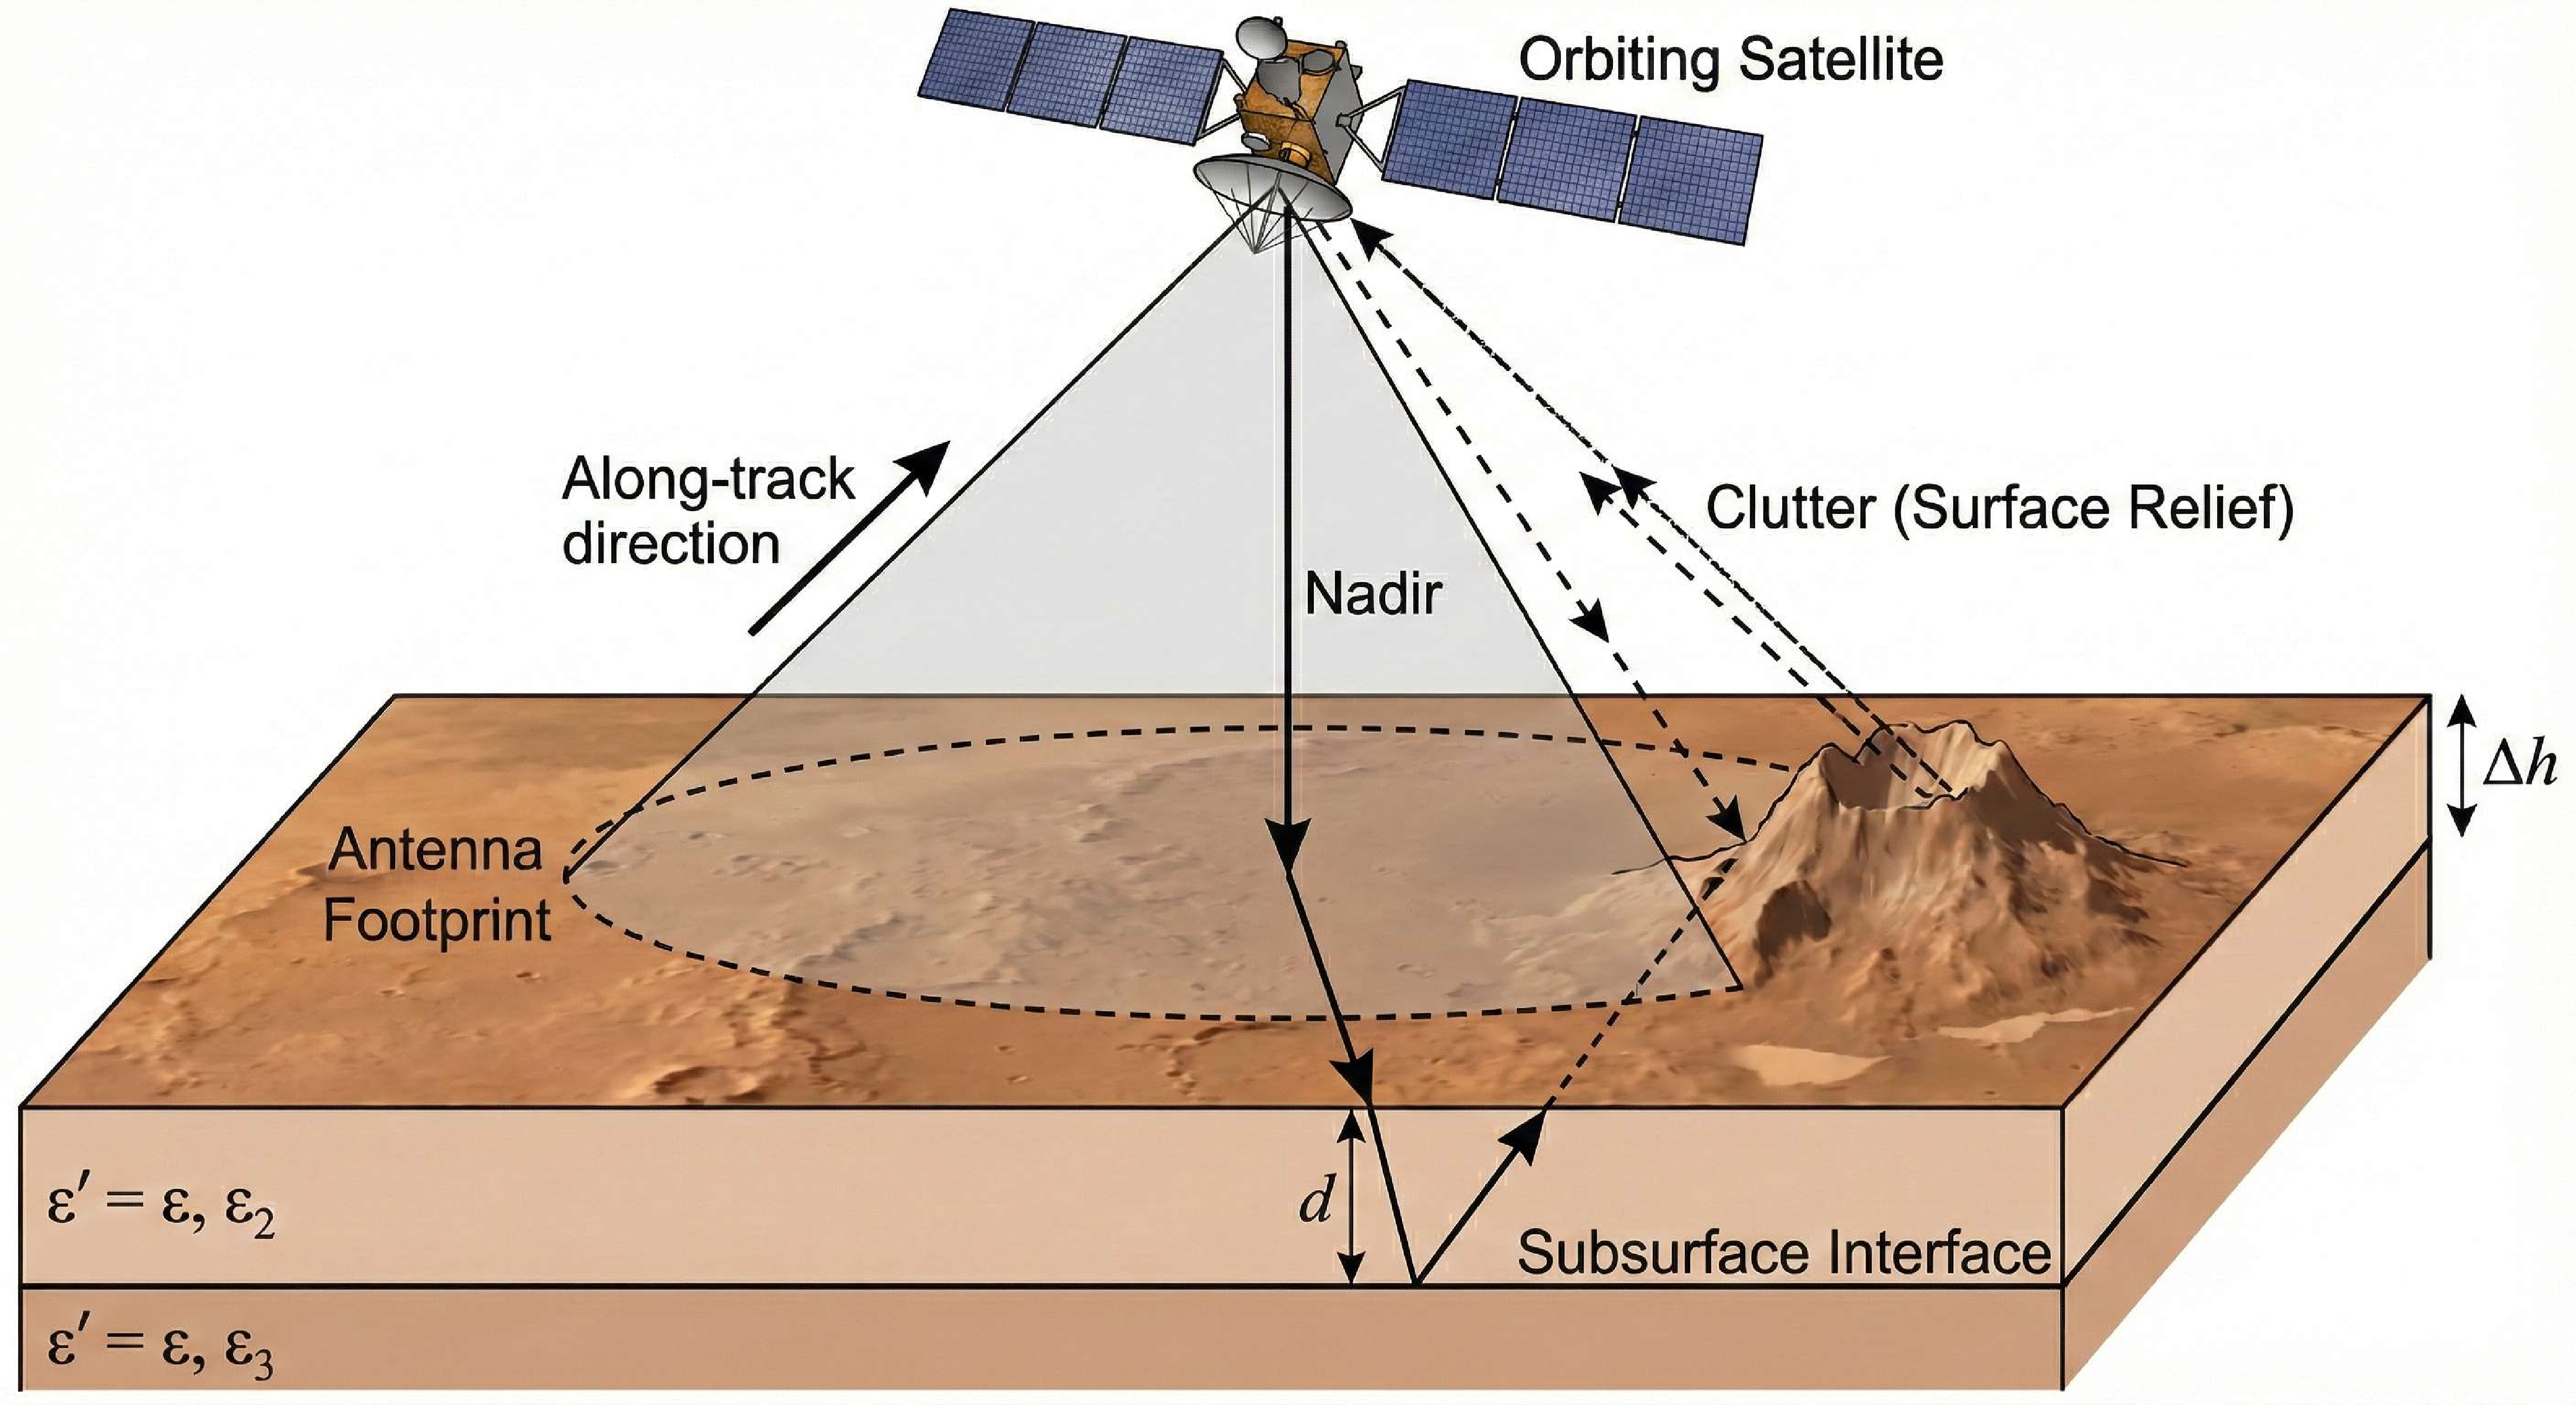
\includegraphics[width=1\linewidth]{images/Gemini_Generated_Image.pdf}
    \caption{Conceptual illustration of a planetary Radar Sounder (RS) acquisition geometry. The nadir-looking instrument transmits pulses that interact with dielectric interfaces in the subsurface (e.g., at depth $d$), returning time-delayed echoes to the receiver \cite{Seu_2007, Daniels_2004}. Due to the finite effective antenna footprint, off-nadir surface topographic features (such as relief with height $\Delta h$) can generate reflections \cite{Seu_2007, foss2017sharad3d}. These ``surface clutter'' signals can arrive at the same time delay as genuine nadir subsurface echoes, complicating data interpretation \cite{foss2017sharad3d, yebasse2025advances}.}
    \label{fig:rs_geometry_clutter}
\end{figure}

